%%%%%%%%%%%%%%%%%%%%%%%%%%%%%%%%%%%%%%%%%%%%%%%%%%%%%%%%%%%%%%%%%%%%%%%%%%%%%%
%
% PROJECT PROPOSAL  DESCRIPTION:
%   A concise description of the main concepts of the proposed project.
%
% RESEARCH:
%   A list of research activities which led to this project.
%
% EXPERIMENTS:
%   A list of the experiments performed which supported the research.
%
%%%%%%%%%%%%%%%%%%%%%%%%%%%%%%%%%%%%%%%%%%%%%%%%%%%%%%%%%%%%%%%%%%%%%%%%%%%%%%%
% Define a single space environment (copied from doublespace.sty)
% e.g. \begin{singlespace}
%         single-spaced text
%      \end{singlespace}

\documentclass[12pt,american]{article}
\usepackage{fullpage}
\usepackage{bbm}
\usepackage{url}
\usepackage{subfigure}
\usepackage{babel}
\usepackage{times}
\usepackage{graphicx}
\usepackage{amssymb}
\usepackage{lscape}
\usepackage{verbatim}
\usepackage{enumerate}
\usepackage{afterpage}
\usepackage{setspace}
\usepackage{listings}
\usepackage{color}
\usepackage{float}
%\usepackage{parskip}

\restylefloat{table}
\lstset{numbers=left,
 frame=single,
 captionpos=b,}

\begin{document}
\thispagestyle{empty} 
\begin{center}
{\em MS Project Proposal}\\
\vspace{.5in}
{\large \bf Buffalo: An Aspect Oriented Programming Framework for C\#}\\
\vspace{.5in}
{\bf Wei Liao}\\
\vfill
\
{\em Committee Chair:} Prof. James E. Heliotis\\
\vspace{0.1in}
%Signature: \line(1,0) {100} Date: \line(250, 0) {100}\\
{\em Reader: } Prof. Fereydoun Kazemian\\
 \vspace{0.1in}
{\em Observer: } Prof. Matthew Fluet\\
 \vspace{0.1in}
Department of Computer Science\\
B. Thomas Golisano College of Computing and Information Sciences \\
Rochester Institute of Technology \\
Rochester, New York \\ [0.3in]
\vspace{0.5in}
\today{}\\
\end{center}
\vfill

%%%%%%%%%%%%%%%%%%%%%%%%%%%%%%%%%%%%%%%%%%%%%%%%%%%%%%%%%%%%%%%%%%%%%%%%%%%%%%%
%%  Collection of useful abbreviations.
\newcommand{\etc} {\emph{etc.\/}}
\newcommand{\etal}{\emph{et~al.\/}}
\newcommand{\eg}  {\emph{e.g.\/}}
\newcommand{\ie}  {\emph{i.e.\/}}
%%%%%%%%%%%%%%%%%%%%%%%%%%%%%%%%%%%%%%%%%%%%%%%%%%%%%%%%%%%%%%%%%%%%%%%%%%%%%%%


%%%%%%%%%%%%%%%%%%%%%%%%%%%%%%%%%%%%%%%%%%%%%%%%%%%%%%%%%%%%%%%%%%%%%%%%%%%%%%%
% Abstract
\section*{Abstract}
Aspect Oriented Programming (AOP) is a paradigm that let programmers isolate and separate cross-cutting concerns from the basis of their program. The concept has not been widely adapted by modern languages, support in toolings such as Integrated Development Environment (IDE) is also rare. In this project we will design and implement a framework called Buffalo that provides AOP functionality for C\# via IL code weaving, and integrate it with the Visual Studio IDE build system.
%%%%%%%%%%%%%%%%%%%%%%%%%%%%%%%%%%%%%%%%%%%%%%%%%%%%%%%%%%%%%%%%%%%%%%%%%%%%%%%
\vfill{}

%%%%%%%%%%%%%%%%%%%%%%%%%%%%%%%%%%%%%%%%%%%%%%%%%%%%%%%%%%%%%%%%%%%%%%%%%%%%%%%
% This is where the main body of the capstone proposal starts
\setcounter{page}{0} 
\newpage{}
%\setlength{\parindent}{1cm}
\section{Introduction}
Object Oriented Programming (OOP) languages have given programmers a lot of freedom in expressing themselves in Object Oriented Design. However, they are still lacking in some areas when it comes to particular software design decision such as cross-cutting concern~\cite{aop}. 

In this project, we will try to solve this type of problem by designing and implementing a framework called "Buffalo" for the C\# platform. We will show that by using Buffalo programmers can separate those concerns from the core of the program, and ultimately be more productive.

In section 2 we will explain the background of the problem, show some examples where the current programming paradigms are not efficient. In section 3, we will explore the existing works and show what have been done. In section 5, we will explain what we propose to do with an overview of the architecture of Buffalo, what we want the end result to be, and how to evaulate it. A tentative roadmap will be given in section 6.

\section{Background}
In this section we will explain more about the cross-cutting problem and how AOP can be used to help.

\subsection{The Problem}
Procedural Language such as C achieves modularity by grouping codes into subroutines, so that they can be reused. Whereas OOP languages, such as JAVA or C\# go one step further, by allowing programmers to abstract real world objects into properties and behaviors. Both paradigms give programmers the ability to make their codes cleaner and more reusable.

While OOP languages offer data abstraction and encapsulation in the form of classes and objects, the usage of declared instances of all these classes could still be scattered throughout different modules of the program. Over time, these tangled cross-cutting relations [1] can become difficult and expensive to maintain. One of the often cited example of such concerns is exception handling: the ability for programs to handle errors or terminate gracefully.

To handle an exception in our code, we usually use the follow try..catch block:

\begin{lstlisting}[caption={try..catch pattern}, label=trycatch]
public double Divide(double num1, double num2) {
   try {
       return num1 / num2;
   } catch (Exception e) {
       //log exception to file, etc
       Utility.LogToFile(e);
   }
}
\end{lstlisting}

The code snippet in Listing~\ref{trycatch} illustrated a few key points. If {\em num2} is 0, the execution will fail, causing an exception to be thrown, and when that happens, execution control is transferred to line 6, where the exception is logged to a file. 

Imagine that if you have 1,000 functions in your program that can potentially throw exceptions, you would have to apply the try..catch block on all of them. And note that the functionality of actually logging the exception is nicely encapsulated in the {\em Utility} object, but it does not change the fact that the code is still repetitive, because {\em Utility.LogToFile(e)} still have to be called in 1,000 different places in the source code. Since an OOP program most likely consists of different modules, this repetitive pattern will cut through and appears in all the them.

What if you need to fine tune this try..catch block to catch a specific exception such as the {\em DivideByZeroException} so your program can act accordingly, or instead of using the {\em Utility} object you want to use a different object to handle the actual logging? In the worst case, you would have to make the change to all 1,000 of your functions.

The problem is how to prevent those cross-cutting concerns from loitering your program. Aspect Oriented Programming techniques~\cite{aop} can be used to cleanly separate such concerns.

\subsection{Aspect-Oriented Programming}
The Aspect Oriented Programming paradigm was first discussed in the 1997 paper~\cite{aop}. When talking about AOP, the following concepts are worth noting:

{\em concern} - the repetitive code that cross-cuts into different modules of the program. Usually the code does not conviently fit into the dominant paradigm of design.

{\em aspect} - the piece of isolated code that can be used to solve the issue of a particluar concern.

{\em join points} - These are the locations through out the program where the concern is leaked into, they are also where the aspect will be applied to solve the concern.

The idea of AOP is fairly simple. We have some code that are duplicated all over the place, making it difficult to maintain, so we need to isolate that duplicate code into a separate single unit. Then we injects that unit of code into all relevant places in a program either at runtime or at compile time, so that the programmers does not have to do it manually in the source code.

In other words, AOP is about injecting code into a program. This is especially handy when programmers don't have access to the original source code.

Beside exception handling, AOP is commonly used in tracing, profiling, security, etc.

\section{Related Work}Most modern programming languages already display some AOP-like properties, but full native support is rare. Delphi Prism is one of them, where the weaving of aspect code happens at compile time~\cite{delphi_prism2010}. AOP can be implemented in a variety of ways. However, just like other programming paradigms, it is most effective and beneficial when it is implemented by the compiler. That makes it a first class citizen like other properties of a language.

\subsection{Compiler Support}

Gregor Kiczales started and led a Xerox PARC team that developed an implementation of AOP for the JAVA platform called AspectJ, as described in a 1997 paper~\cite{aop}. AspectJ is an extension to the JAVA compiler. It is a language in and of itself, with its own specific syntax and usages, and even its own compiler. It produces JAVA VM compatible binary. Some people hopes that AspectJ will eventually be merged with the JAVA compiler instead of being just an extendsion~\cite{aspectj_faq}. Still, AspectJ integrates nicely with JAVA, especially when used with its own plugin AJDT in the Eclipse IDE.

AspectJ can introduce new features to a program, as well as the modification of it. It provides the {\em aspect} keyword to denote a piece of code as the advice code, usage is similar to the {\em class} keyword in JAVA.

\begin{lstlisting}[caption={sample AspectJ code}, label=aspecjcode]
public aspect MyAspectJ {
   public int Sorter.Count() {
      //do something here
   }
   pointcut doSomething() : call (* * (..));
   before() : doSomething() {
      //do something before calling the actual function
   }
}
\end{lstlisting}

The example in Listing~\ref{aspecjcode} showed how an aspect is defined in AspectJ. Suppose we have a class named {\em Sorter}, and we want to add a new method to it but we don't have access to the source code. In AspectJ, we can introduce a brand new method {\em Count} to it, as shown in line 2-4. The pointcut {\em doSomething} does a match to find all matching functions regardless of access priviledge, names or parameters, which means pretty much every function in the program. Line 6-8 means before the matched functions are executed, the block of code in line 7 is executed first. This effectively creates a hook into every single function in a program, allowing programmers to inject custom code into it.

Behind the scene, AspectJ pieces everything together using bytecode weaving. After JAVA compiles the source, AspectJ takes the classes and aspects in bytecode form and weaves them together, producing new .class files that can be loaded onto the virtual machine.

Despite Eclipse's claim that AspectJ is very easy to learn, one of the disadvantages of AspectJ, as Listing~\ref{aspecjcode} shows, is that the syntax is somewhat different from a normal JAVA program, making the learning curve much deeper. But we agree that once we get used to it, AspectJ can be a really powerful tool for a programmer~\cite{aspectj_text}.

\subsection{Framework Support}

AspectJ is one of the few compilers that does AOP, that is good news for JAVA programmer. For the vast majority of other programming languages out there, AOP support is provided via frameworks. This is especially true on the C\# platform~\cite{aopcs}, where Microsoft has indicated that they will not be integrating AOP support into the C\# compiler anytime soon~\cite{mastermind_text}. There was a project called Eos developed at the University of Virginia, which was an aspect oriented extension for C\#, but it had been discontinued years ago~\cite{eos_site, eos}.

There are a number of frameworks available for the C\# platform, they come in various flavors and implemented with different techniques. The different approaches each has its own advantages and disadvantage.

One of the most common implementation involves the usage of a proxy, where the client does not interact with the objects directly, rather everything goes through the proxy.

\begin{figure}[here]
  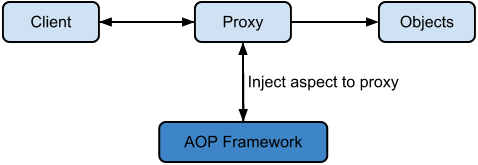
\includegraphics[scale=0.70]{proxy.png}
  \centering
  \caption{AOP framework using proxy\label{proxy_model}}
\end{figure}

Using the proxy provides an opportunity for code injection. The advantage of this approach is relative ease of implementation. It is also limiting since in order for the proxy to work, both the proxy and the target object must implement the same interface, therefore the aspect injection point can only occur in the exposed functions for the interface. As this requires reflection at runtime to generate the proxy, it also adds overhead, so performance might not be as good as other approaches.

Another approach is similar to AspectJ, where bytecode weaving is used, but without the extra complexity of a new syntax and language. The commercial product PostSharp~\cite{postsharp} is such an example, where aspect weaving happens post compilation by rewriting the MSIL instruction set. PostSharp uses only the standard C\# language with attribute used for advice codes. The advantage is ease of use, as developers already familiar with C\# will have little to no learning curve at all. And since aspect is woven in the assembly, the runtime incurs no overhead for reflection, and therefore performance is not compromised. The disadvantage is that, since it has to work with MSIL instruction set, it is very low level and therefore the most difficult to implement.

Some frameworks use static weaving~\cite{aspectcs}, where the source files are pre-processed to include all the relevant aspect code. Then the C\# compiler takes over and does the compilation normally. This has the advantage of post compilation weaving but not the complexity of working with MSIL instruction set. On the other hand, a parsar generator has to be developed to efficiently parse the source files.

\section{Hypothesis}
The OOP paradigm cannot efficiently solve the cross-cutting problem. Even though the C\# compiler will not support the AOP paradigm, we can still archieve the same goal by performing the separation of concerns via Buffalo.

We can further make the developer's life easier by hooking up Buffalo with the MSBuild system to perform automatic aspect weaving. With zero configuration requirement, developers can just focus on creating the aspects to deal with the problems.

\section{Approach and Methodology}
In this section we will give an overview of the architecture of Buffalo, the tools and approaches we will be using to implement it.

\subsection{Architecture Overview}
The approach we plan to take is to perform compile time weaving. Figure~\ref{buffalo_model} shows an overview of how Buffalo will fit in the overall C\# compilation process.

\begin{figure}[here]
  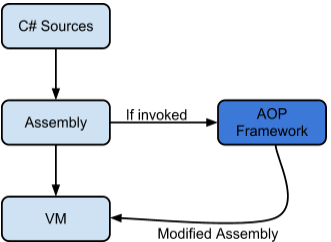
\includegraphics[scale=0.70]{model_overview.png}
  \centering
  \caption{Buffalo model overview\label{buffalo_model}}
\end{figure}

\subsection{Compile Time Weaving}
As shown in Figure~\ref{buffalo_model}, the C\# compiler compiles the source files into an assembly, this assembly is then fed into Buffalo. Buffalo takes apart the assembly using reflection to find all the defined {\em aspects} and possible {\em pointcuts}, then weave them together at the right places by rewriting the MSIL instruction set, and finally produces a new assembly.

Once C\# finishes the compilation, the control is transferred to Buffalo. This is archieved by creating a hook into the MSBuild system. If Buffalo detects any {\em aspects} defined in the input assembly, and that the {\em aspects} are being applied, then weaving will take place, otherwise the whole process will simply be ignored.

\subsection{Intended Usage}
From the Visual Studio IDE, developer can use Buffalo by creating a custom C\# attribue, extending a Buffalo interface IAspect (subject to change), for example:

\begin{lstlisting}[caption={Buffalo aspect}, label=buffalocode]
public class CatchException : System.Attribute, IAspect {
   public void OnException(Exception e) {
       Utility.LogToFile(e);
   } 
}
\end{lstlisting}

The cross-cutting concerns is now cleanly separated into a cutom attribute {\em CatchException}. It will be treated as an aspect by Buffalo, any change made to it will be propagated to all the annontated functions. To use this aspect, simply treat it like a regular attribute and apply it to any method, class or assembly.

\begin{lstlisting}[caption={applying Buffalo aspect}, label=applybuffalo]
[CatchException]
public double Divide(double num1, double num2) {
   return num1 / num2;
}
\end{lstlisting}

As the code snippets in Listing~\ref{applybuffalo} shows, by applying this attribute to a function, the repetitive try..catch block is no longer necessary. The target code is much shorter and cleaner. 

The real benefit will be evident when an aspect is applied to a large number of functions, or asemblies. For example, if we want every function in every class to be able to catch exception we can apply the attribute to the assembly:

\begin{lstlisting}[caption={applying Buffalo aspect on an assembly}, label=applybuffaloassembly]
[assembly:CatchException]
namespace MyAssembly {
   public class MyClass {
      public double Divide(double num1, double num2) {
         return num1 / num2;
      }
      //other functions...
   }
   //other classes...
}
\end{lstlisting}

By applying the attribute on the assembly level, a single line of code, will effectively allow every function to have exception handling capability. This will be a huge developer productivity gain.

\subsection{Platform, Languages and Tools}
This project will be developed using C\# and Visual Studio 2010, on Windows 7. For IL rewriting several options are available. One is to use the Reflection.Emit library that comes with the .NET Framework. However all research indicates that this library represents only a subset of the MSIL instruction set.

Another option is to use the Profiler API by Microsoft, but this API is intended as a debugging feature, therefore is unsuitable for production environment.

While we can opt to invest the time on learning and developing a custom MSIL rewriter, we are afraid that that in itself is a bigger project than Buffalo~\cite{msil_text}. Mono is an open source implementation of the C\# compiler, Cecil is a project within Mono that provides MSIL rewriting. Cecil provides very low level API for working with MSIL. Preliminary evaluation of the tool suggests it is pretty feature complete and flexible enough to satisfy our requirement. However, documentation for Cecil is next to non-existent, so the learning curve is expected to be deep.

The following utility tools will also be heavily used during development: ILSpy, ILDASM and PEVerify. ILSpy is an open source application that dis-assembles C\# assembly to show IL instructions. ILDASM does the same thing but comes from Microsoft .NET Framework. PEVerify is a Microsoft Windows SDK tool, it will be used to ensure that the modified assembly we will produce is valid, as this is not verified by Cecil.

\subsection{Measurement}
To evalulate Buffalo, we will show that with Buffalo, code duplication can be reduced. The cross-cutting concern will be separated into single unit of code where it will be easy to maintain. We will use the {\em Call Hierarchy} feature of Visual Studio to show how many calls are issued before and after IL rewrite with Buffalo. 

The line count of code a developer has to write will also be reduced considerably. As a result the code will be cleaner and easier to look at. This can also be translated directly into an estimation of development cost savings. We will compare line counts before and after IL code rewrite by Buffalo using the {\em Code Analysis} function provided by Visual Studio.

\section{Roadmap}
Table~\ref{tab:roadmap_tbl} shows the tentative schedule for the major phases of this project.

\begin{table}[H]
\centering
\begin{tabular}{|l|l|l|}
\hline
Date & Action & Status\\
\hline
07/07/2012 & Pre-Proposal & Accepted\\
07/09/2012 & Proposal & In-progress\\
07/20/2012 & Begin development of Buffalo & In-progress\\
09/10/2012 & Finish development, start testing and analysis & - \\
09/27/2012 & Finish report & - \\
10/10/2012 & Defense & - \\
\hline
\end{tabular}
\caption{Timeline}
\label{tab:roadmap_tbl}
\end{table}

%%%%%%%%%%%%%%%%%%%%%%%%%%%%%%%%%%%%%%%%%%%%%%%%%%%%%%%%%%%%%%%%%%%%%%%%%%%%%%%

%%%%%%%%%%%%%%%%%%%%%%%%%%%%%%%%%%%%%%%%%%%%%%%%%%%%%%%%%%%%%%%%%%%%%%%%%%%%%%%
%\bibliographystyle{plain}
\bibliographystyle{unsrt}
% Single space the bibliography to save space.
\singlespacing
\bibliography{Proposal}
%%%%%%%%%%%%%%%%%%%%%%%%%%%%%%%%%%%%%%%%%%%%%%%%%%%%%%%%%%%%%%%%%%%%%%%%%%%%%%%


\end{document}
